\chapter{Requirement Specifications} \label{cap:reqs}

Our purposed system is a "Carpool" application wic is a ride saring application designed just for students. Students can login or signup to tis application only via university email. We made sure tat only enrolled students in a university use tis application. Te application involves functional and non-functional functionalities tat must be performed by te system.

\subsection{Functional Requirements}

\begin{center}

\centering
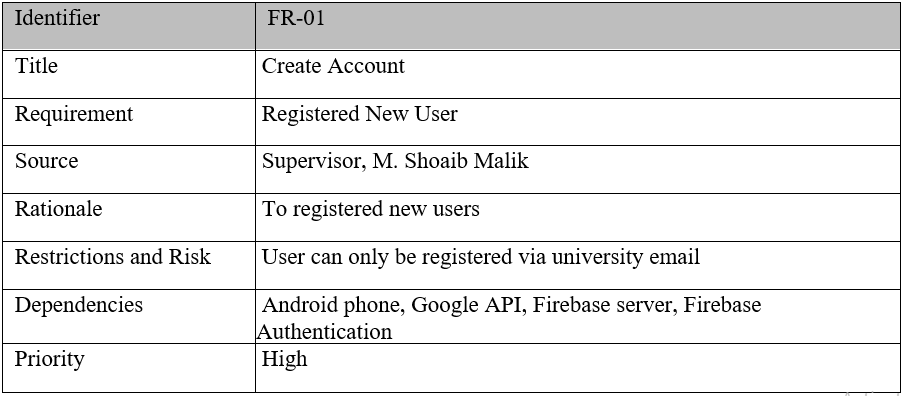
\includegraphics[width=1.0\textwidth]{TableFR1}
\captionof{table}{Functional Requirement - 01}
\end{center}

\begin{center}

\centering
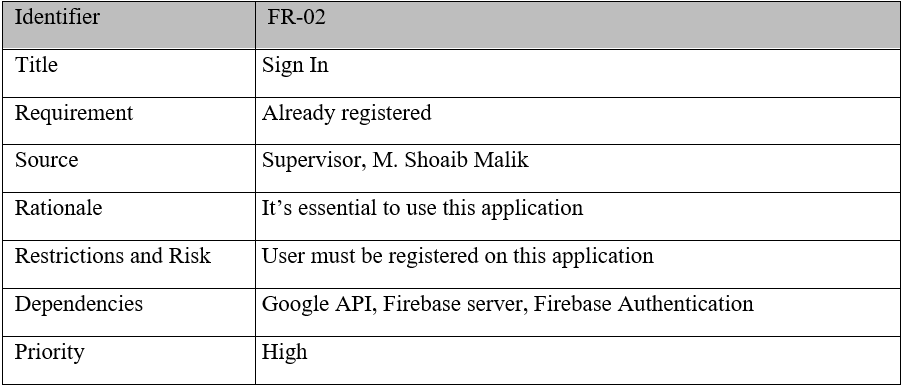
\includegraphics[width=1.0\textwidth]{TableFR2}
\captionof{table}{Functional Requirement - 02}
\end{center}

\begin{center}

\centering
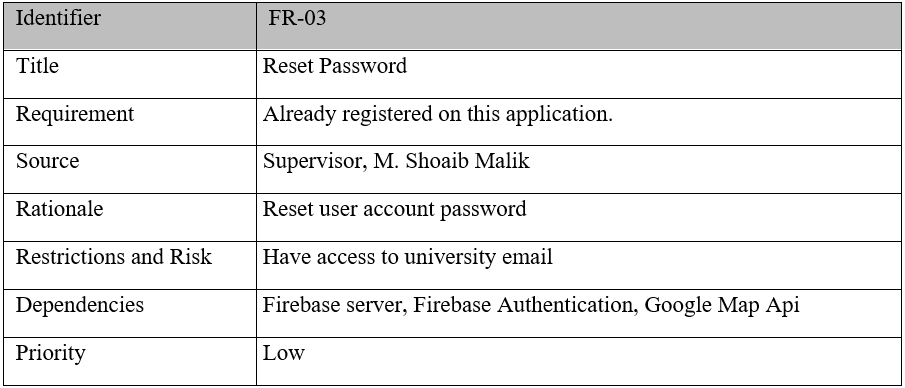
\includegraphics[width=1.0\textwidth]{TableFR3}
\captionof{table}{Functional Requirement - 03}
\end{center}

\begin{center}

\centering
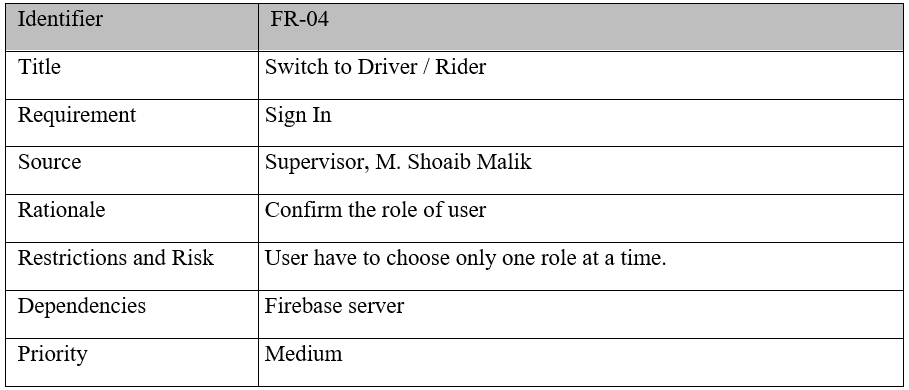
\includegraphics[width=1.0\textwidth]{TableFR4}
\captionof{table}{Functional Requirement - 04}
\end{center}

\begin{center}

\centering
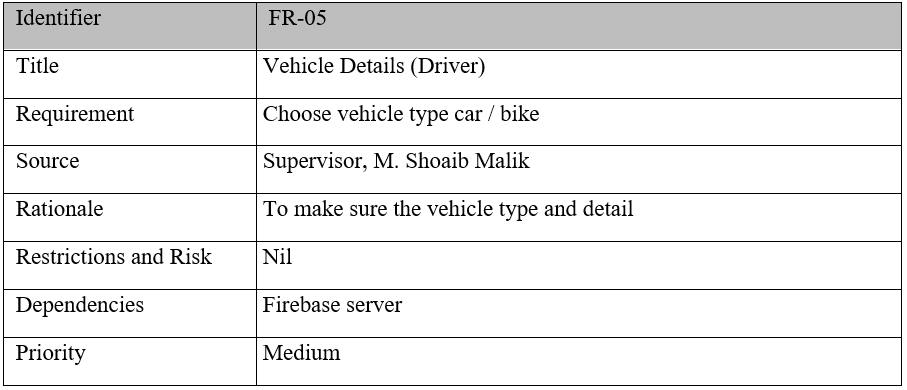
\includegraphics[width=1.0\textwidth]{TableFR5}
\captionof{table}{Functional Requirement - 05}
\end{center}

\begin{center}

\centering
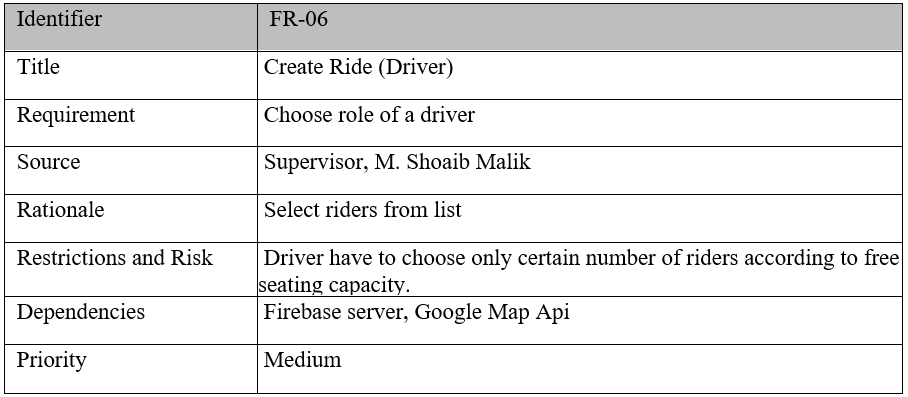
\includegraphics[width=1.0\textwidth]{TableFR6}
\captionof{table}{Functional Requirement - 06}
\end{center}

\begin{center}

\centering
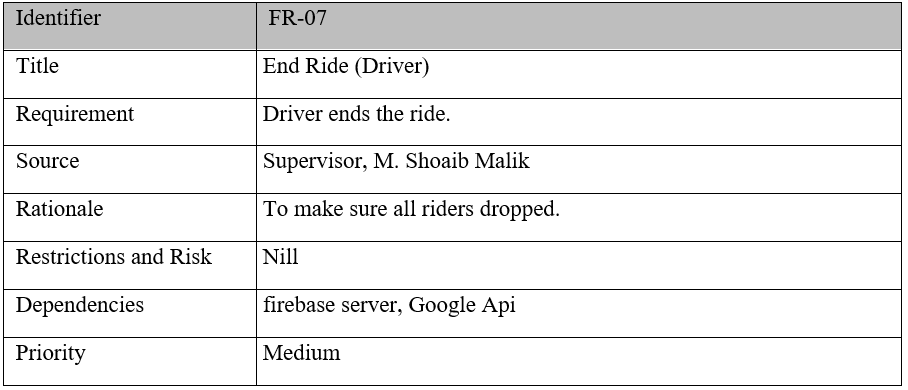
\includegraphics[width=1.0\textwidth]{TableFR7}
\captionof{table}{Functional Requirement - 07}
\end{center}

\begin{center}

\centering
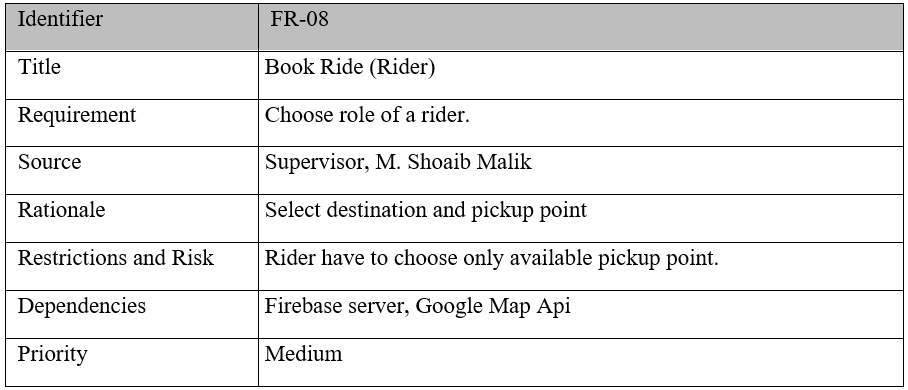
\includegraphics[width=1.0\textwidth]{TableFR8}
\captionof{table}{Functional Requirement - 08}
\end{center}

\begin{center}

\centering
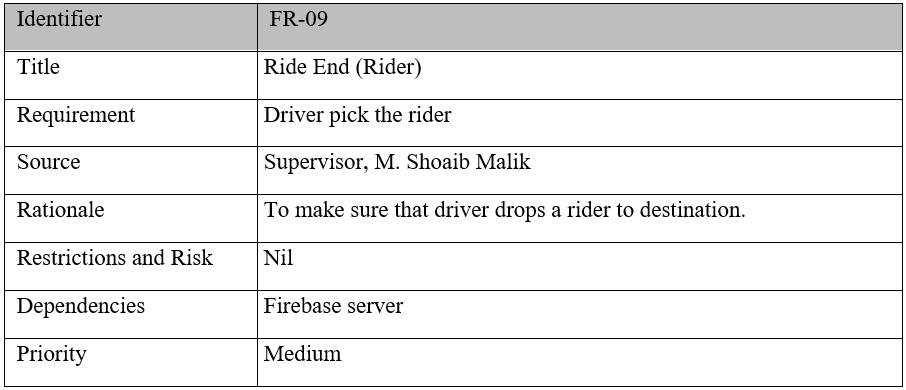
\includegraphics[width=1.0\textwidth]{TableFR9}
\captionof{table}{Functional Requirement - 09}
\end{center}


\subsection{Non-Functional Requirements} 

\begin{center}
\centering
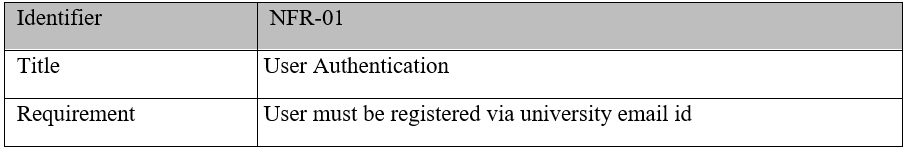
\includegraphics[width=1.0\textwidth]{TableNFR1}
\captionof{table}{Non-Functional Requirement - 01}
\end{center}

\begin{center}

\centering
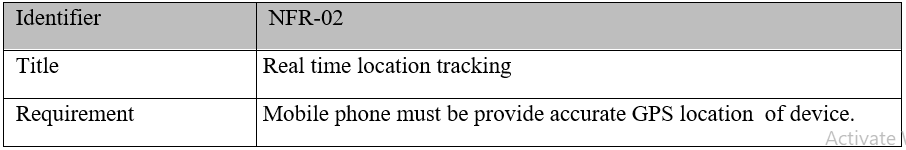
\includegraphics[width=1.0\textwidth]{TableNFR2}
\captionof{table}{Non-Functional Requirement - 02}
\end{center}

\begin{center}

\centering
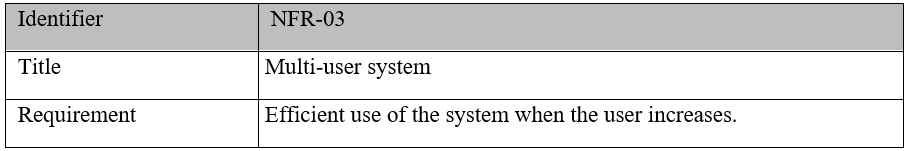
\includegraphics[width=1.0\textwidth]{TableNFR3}
\captionof{table}{Non-Functional Requirement - 03}
\end{center}

\begin{center}

\centering
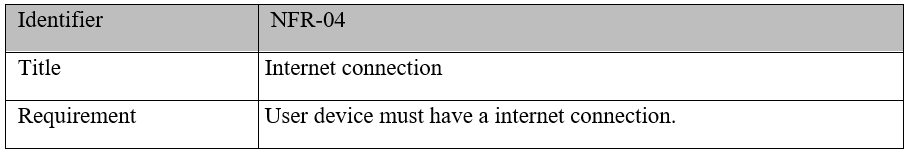
\includegraphics[width=1.0\textwidth]{TableNFR4}
\captionof{table}{Non-Functional Requirement - 04}
\end{center}

\begin{center}

\centering
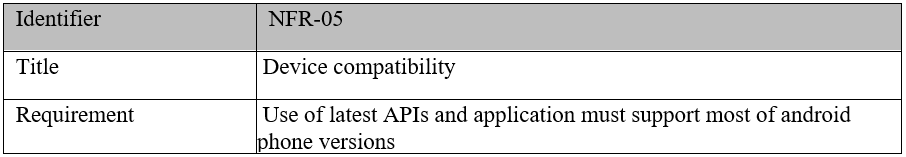
\includegraphics[width=1.0\textwidth]{TableNFR5}
\captionof{table}{Non-Functional Requirement - 05}
\end{center}

\begin{center}

\centering
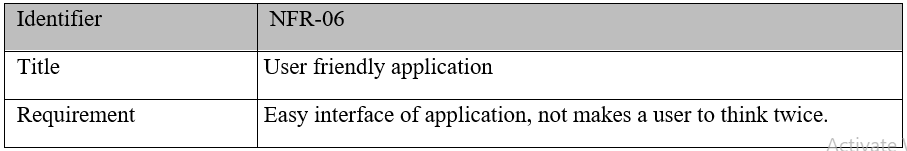
\includegraphics[width=1.0\textwidth]{TableNFR6}
\captionof{table}{Non-Functional Requirement - 06}
\end{center}

\begin{center}

\centering
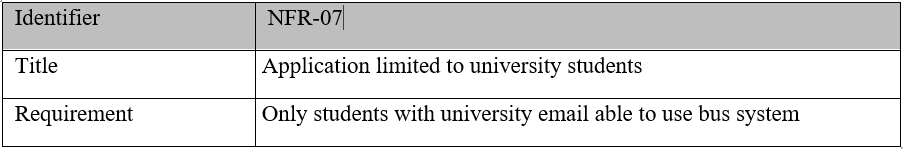
\includegraphics[width=1.0\textwidth]{TableNFR7}
\captionof{table}{Non-Functional Requirement - 07}
\end{center}


\section{Use Cases}

\begin{center}
\centering
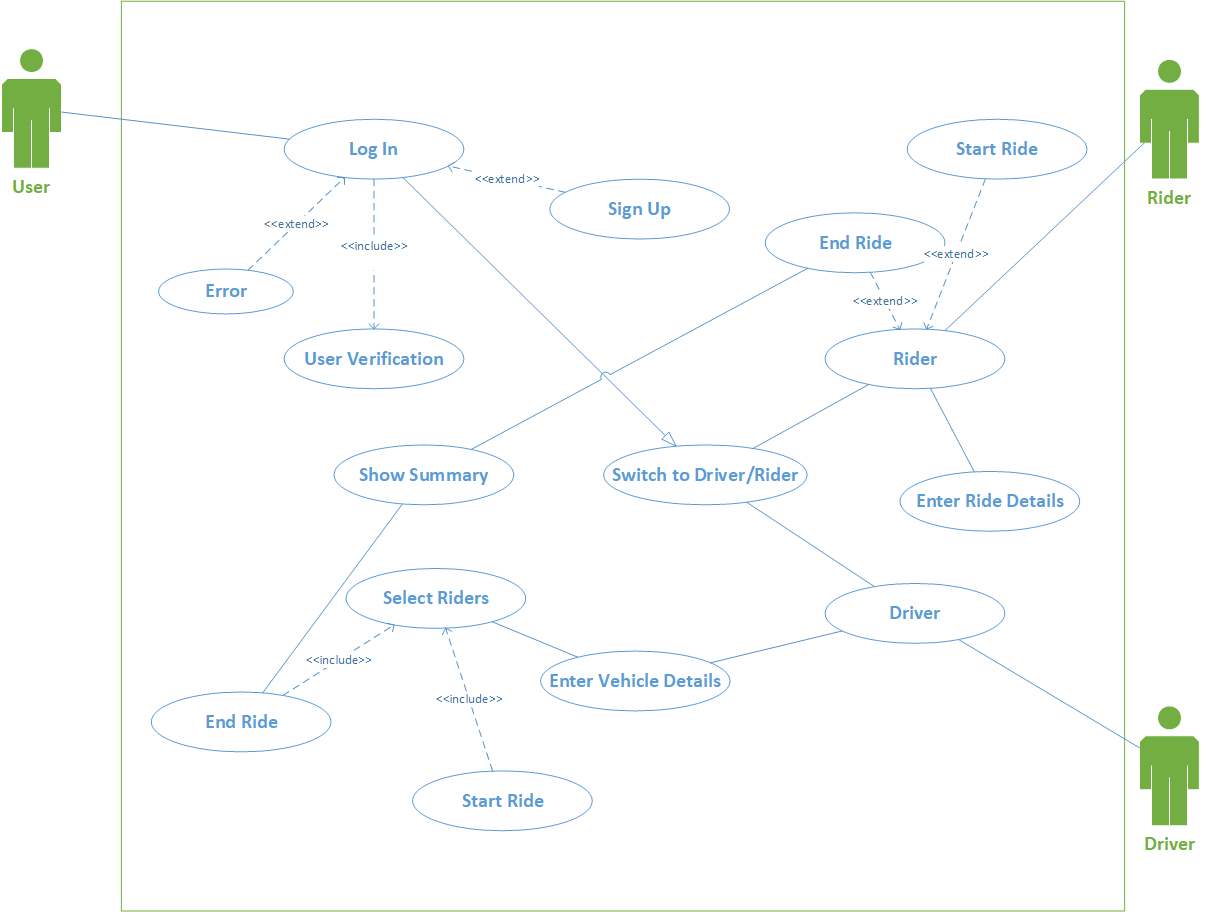
\includegraphics[width=1.0\textwidth]{UseCaseDiagram}
\captionof{figure}{Use Case Diagram}
\label{fig:UseCaseDiagram}
\end{center}

\begin{center}
\centering
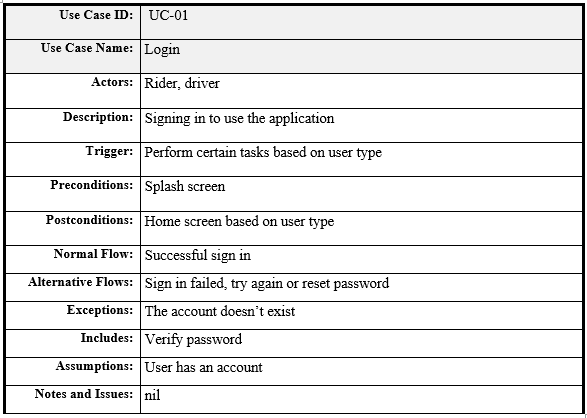
\includegraphics[width=1.0\textwidth]{TableUC1}
\captionof{table}{Use Case - 01}
\end{center}
\begin{center}

\centering
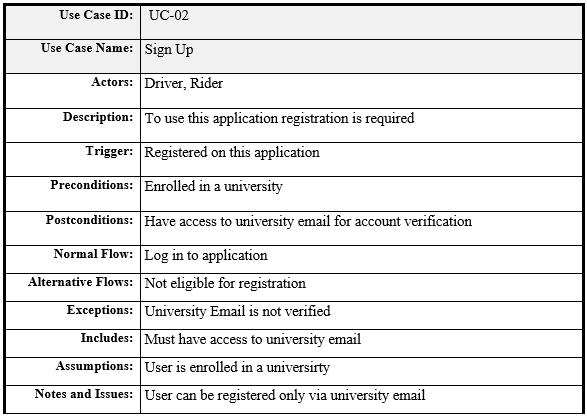
\includegraphics[width=1.0\textwidth]{TableUC2}
\captionof{table}{Use Case - 02}
\end{center}

\begin{center}

\centering
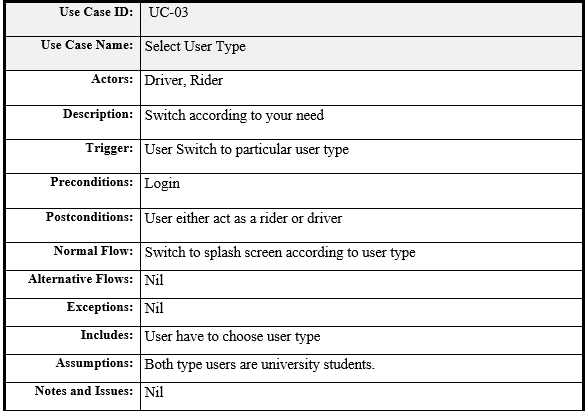
\includegraphics[width=1.0\textwidth]{TableUC3}
\captionof{table}{Use Case - 03}
\end{center}

\begin{center}

\centering
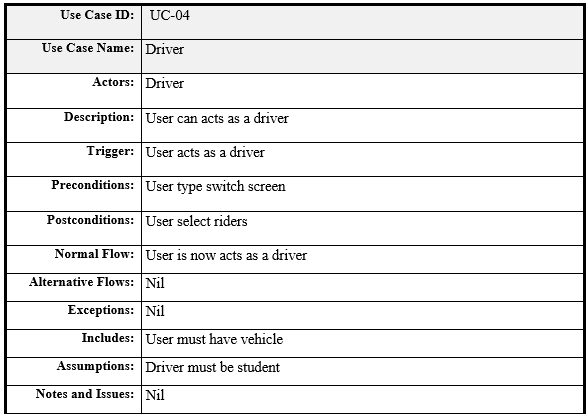
\includegraphics[width=1.0\textwidth]{TableUC4}
\captionof{table}{Use Case - 04}
\end{center}

\begin{center}

\centering
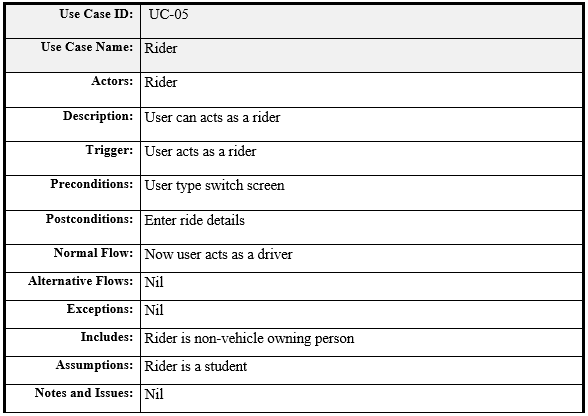
\includegraphics[width=1.0\textwidth]{TableUC5}
\captionof{table}{Use Case - 05}
\end{center}

\begin{center}

\centering
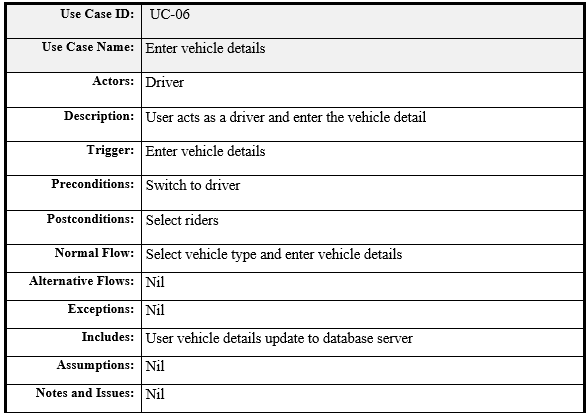
\includegraphics[width=1.0\textwidth]{TableUC6}
\captionof{table}{Use Case - 06}
\end{center}

\begin{center}

\centering
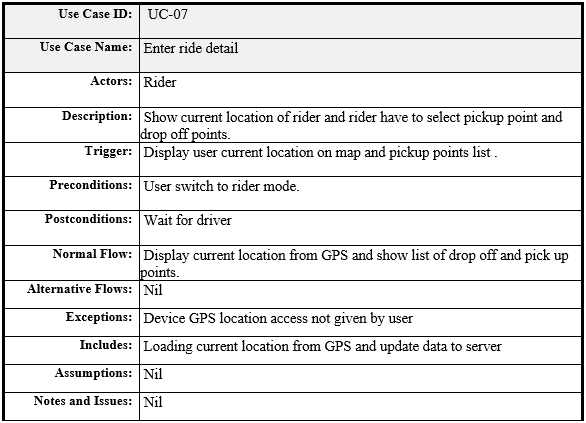
\includegraphics[width=1.0\textwidth]{TableUC7}
\captionof{table}{Use Case - 07}
\end{center}

\begin{center}

\centering
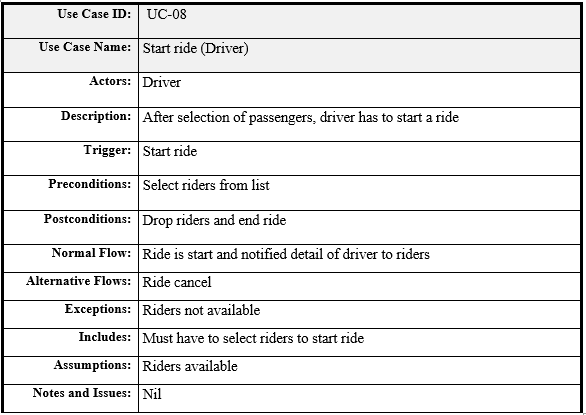
\includegraphics[width=1.0\textwidth]{TableUC8}
\captionof{table}{Use Case - 08}
\end{center}

\begin{center}

\centering
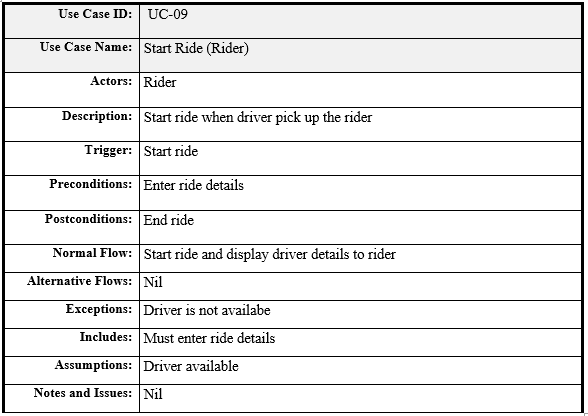
\includegraphics[width=1.0\textwidth]{TableUC9}
\captionof{table}{Use Case - 09}
\end{center}

\begin{center}

\centering
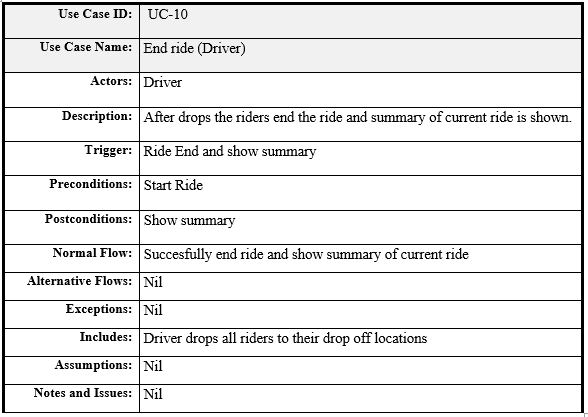
\includegraphics[width=1.0\textwidth]{TableUC10}
\captionof{table}{Use Case - 10}
\end{center}

\begin{center}
	
\centering
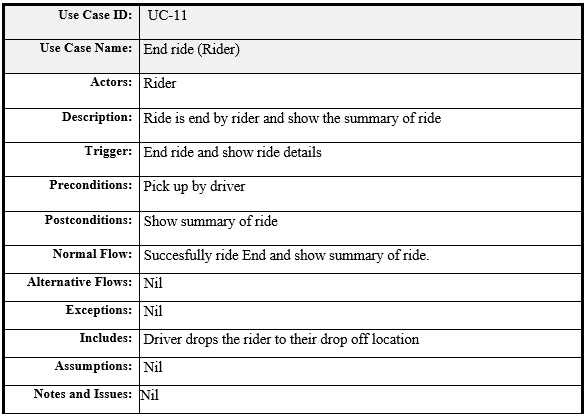
\includegraphics[width=1.0\textwidth]{TableUC11}
\captionof{table}{Use Case - 11}
\end{center}
 

